\documentclass[14pt,a4paper]{extreport}

\usepackage[T2A]{fontenc}
\usepackage[utf8]{inputenc}
\usepackage[russian]{babel}
\usepackage{amsmath}
\usepackage{graphicx}
\usepackage{geometry}
\geometry{left=2cm,right=2cm,top=2cm,bottom=2cm}
\usepackage{listings}
\usepackage{xcolor}
\usepackage{caption}
\usepackage{hyperref}
\usepackage{float}

% Настройка листингов для Python
\lstset{
    language=Python,
    basicstyle=\ttfamily\footnotesize,
    numbers=left,
    numberstyle=\tiny\color{gray},
    stepnumber=1,
    numbersep=8pt,
    showstringspaces=false,
    breaklines=true,
    frame=single,
    tabsize=4,
    captionpos=t,
    extendedchars=true,
    literate={а}{{\selectfont\char224}}1
             {б}{{\selectfont\char225}}1
             {в}{{\selectfont\char226}}1
             {г}{{\selectfont\char227}}1
             {д}{{\selectfont\char228}}1
             {е}{{\selectfont\char229}}1
             {ё}{{\"e}}1
             {ж}{{\selectfont\char230}}1
             {з}{{\selectfont\char231}}1
             {и}{{\selectfont\char232}}1
             {й}{{\selectfont\char233}}1
             {к}{{\selectfont\char234}}1
             {л}{{\selectfont\char235}}1
             {м}{{\selectfont\char236}}1
             {н}{{\selectfont\char237}}1
             {о}{{\selectfont\char238}}1
             {п}{{\selectfont\char239}}1
             {р}{{\selectfont\char240}}1
             {с}{{\selectfont\char241}}1
             {т}{{\selectfont\char242}}1
             {у}{{\selectfont\char243}}1
             {ф}{{\selectfont\char244}}1
             {х}{{\selectfont\char245}}1
             {ц}{{\selectfont\char246}}1
             {ч}{{\selectfont\char247}}1
             {ш}{{\selectfont\char248}}1
             {щ}{{\selectfont\char249}}1
             {ъ}{{\selectfont\char250}}1
             {ы}{{\selectfont\char251}}1
             {ь}{{\selectfont\char252}}1
             {э}{{\selectfont\char253}}1
             {ю}{{\selectfont\char254}}1
             {я}{{\selectfont\char255}}1
             {А}{{\selectfont\char192}}1
             {Б}{{\selectfont\char193}}1
             {В}{{\selectfont\char194}}1
             {Г}{{\selectfont\char195}}1
             {Д}{{\selectfont\char196}}1
             {Е}{{\selectfont\char197}}1
             {Ё}{{\"E}}1
             {Ж}{{\selectfont\char198}}1
             {З}{{\selectfont\char199}}1
             {И}{{\selectfont\char200}}1
             {Й}{{\selectfont\char201}}1
             {К}{{\selectfont\char202}}1
             {Л}{{\selectfont\char203}}1
             {М}{{\selectfont\char204}}1
             {Н}{{\selectfont\char205}}1
             {О}{{\selectfont\char206}}1
             {П}{{\selectfont\char207}}1
             {Р}{{\selectfont\char208}}1
             {С}{{\selectfont\char209}}1
             {Т}{{\selectfont\char210}}1
             {У}{{\selectfont\char211}}1
             {Ф}{{\selectfont\char212}}1
             {Х}{{\selectfont\char213}}1
             {Ц}{{\selectfont\char214}}1
             {Ч}{{\selectfont\char215}}1
             {Ш}{{\selectfont\char216}}1
             {Щ}{{\selectfont\char217}}1
             {Ъ}{{\selectfont\char218}}1
             {Ы}{{\selectfont\char219}}1
             {Ь}{{\selectfont\char220}}1
             {Э}{{\selectfont\char221}}1
             {Ю}{{\selectfont\char222}}1
             {Я}{{\selectfont\char223}}1
}

\begin{document}

% ===== ТИТУЛЬНЫЙ ЛИСТ =====
\begin{titlepage}
\begin{center}
\large
Министерство науки и высшего образования Российской Федерации\\[5pt]
Федеральное государственное автономное образовательное учреждение\\
высшего образования\\[5pt]
\textbf{«Национальный исследовательский университет ИТМО»}\\[20pt]
\Large
\textbf{Курсовая работа}\\[5pt]
по дисциплине «Объектно-ориентированное программирование»\\[20pt]
\LARGE
\textbf{Учет внутриофисных расходов}\\[40pt]
\end{center}

\begin{flushright}
Выполнил:\\
студент группы \_\_\_\_\_\_\_\_\_\_\\
\_\_\_\_\_\_\_\_\_\_\_\_\_\_\_\_\_\_\_\_\_\_\\
Проверил:\\
\_\_\_\_\_\_\_\_\_\_\_\_\_\_\_\_\_\_\_\_\_\_\\
\end{flushright}

\vfill
\begin{center}
Санкт-Петербург\\
2024
\end{center}
\end{titlepage}

% ===== ОГЛАВЛЕНИЕ =====
\tableofcontents
\newpage

% ===== ВВЕДЕНИЕ =====
\chapter{Введение}

Целью данной курсовой работы является разработка приложения на языке Python с графическим интерфейсом PyQt5 для автоматизации учёта внутриофисных расходов частной фирмы. Приложение реализует объектно-ориентированный подход к моделированию предметной области и поддерживает сохранение/загрузку данных в формате XML.

Предметная область включает три сущности:
\begin{itemize}
    \item \textbf{Отделы} (Название, Количество сотрудников)
    \item \textbf{Виды расходов} (Название, Описание, Предельная норма)
    \item \textbf{Расходы} (Вид расхода, Отдел, Сумма, Дата)
\end{itemize}

Приложение построено по многослойной архитектуре: слой данных (классы-сущности и списки), слой хранения (чтение/запись XML), слой графического интерфейса (таблицы, формы редактирования, страницы с вкладками).

\chapter{Задание 1: Реализация классов сущностей}

\section{Пояснение к выполнению Задания 1}

Согласно предоставленным источникам, первым этапом разработки является создание базовых классов, моделирующих сущности предметной области. В основе иерархии лежит класс \texttt{general}, который обрабатывает общие атрибуты \texttt{code} и \texttt{name}, используя принцип обобщения. Все остальные сущности наследуются от него, добавляя специфические атрибуты через методы доступа (set/get), обеспечивающие инкапсуляцию данных.

\subsection{Модуль \texttt{general.py}}

Этот базовый класс обрабатывает общие атрибуты \texttt{code} и \texttt{name}, используя принцип обобщения.

\lstinputlisting[label=lst:general,caption=Модуль \texttt{general.py} --- базовый класс сущностей]{general.py}

\subsection{Модуль \texttt{department.py}}

Класс для сущности «Отдел» (\texttt{department}), наследуемый от \texttt{general}. Добавляет атрибут \texttt{employees} (количество сотрудников).

\lstinputlisting[label=lst:department,caption=Модуль \texttt{department.py} --- сущность «Отдел»]{department.py}

\subsection{Модуль \texttt{expensetype.py}}

Класс для сущности «Вид расхода» (\texttt{expensetype}), включающий описание и предельную норму.

\lstinputlisting[label=lst:expensetype,caption=Модуль \texttt{expensetype.py} --- сущность «Вид расхода»]{expensetype.py}

\subsection{Модуль \texttt{expense.py}}

Класс «Расход» (\texttt{expense}), который связывает отдел и вид расхода через агрегацию. Содержит поля \texttt{amount} (сумма) и \texttt{date} (дата), а также вспомогательные методы для получения названий связанных объектов.

\lstinputlisting[label=lst:expense,caption=Модуль \texttt{expense.py} --- сущность «Расход»]{expense.py}

\section{UML-диаграмма классов сущностей}

На рисунке~\ref{fig:uml1} представлена диаграмма классов, отражающая отношения наследования и агрегации между сущностями. Класс \texttt{expense} агрегирует как \texttt{department}, так и \texttt{expensetype}, в то время как все три наследуют от \texttt{general}.

\begin{figure}[H]
\centering
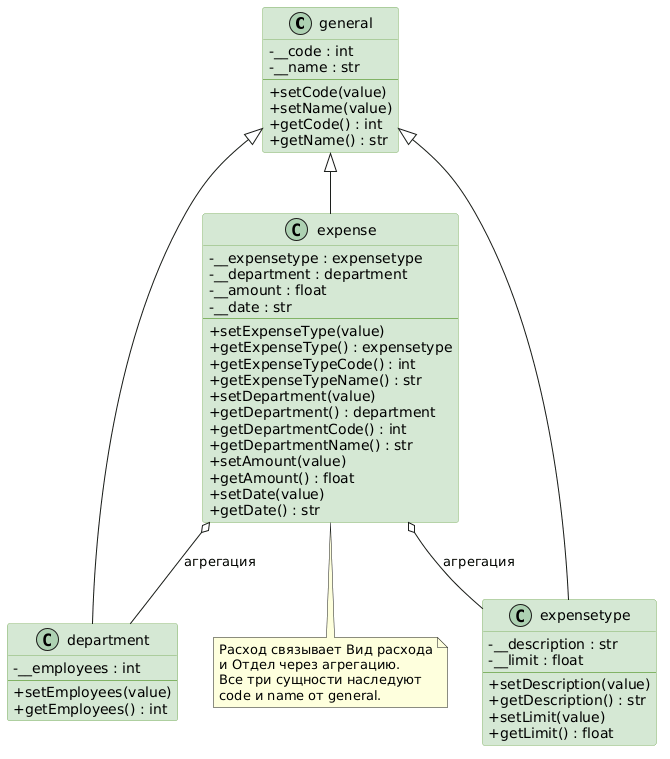
\includegraphics[width=0.85\textwidth]{screenshots/uml_entities.png}
\caption{UML-диаграмма классов сущностей}
\label{fig:uml1}
\end{figure}

\chapter{Задание 2: Реализация системы хранения данных}

\section{Пояснение к выполнению Задания 2}

Согласно источникам, реализация системы хранения данных строится на следующих принципах:

\begin{enumerate}
    \item \textbf{Специализированные списки:} Для каждой сущности создаются классы-списки (наследники \texttt{generalList}), которые обеспечивают контроль типов и фабричные методы для создания объектов.
    \item \textbf{Центральный управляющий класс:} Создаётся класс \texttt{accounting}, который объединяет все списки и координирует работу с ними.
    \item \textbf{Иерархия классов данных:} Базовый класс \texttt{data} определяет общие атрибуты для работы с файлами, а его наследник \texttt{dataxml} реализует конкретную логику чтения и записи XML через библиотеку \texttt{xml.dom.minidom}.
\end{enumerate}

\subsection{Модуль \texttt{generallist.py}}

Базовый класс списка, предоставляющий общие методы: поиск по коду, получение нового кода, добавление/удаление элементов.

\lstinputlisting[label=lst:generallist,caption=Модуль \texttt{generallist.py} --- базовый класс списка]{generallist.py}

\subsection{Модуль \texttt{departmentlist.py}}

Класс для управления коллекцией объектов \texttt{department}. Переопределяет \texttt{appendItem} с проверкой типа и добавляет фабричные методы \texttt{createItem} и \texttt{newItem}.

\lstinputlisting[label=lst:departmentlist,caption=Модуль \texttt{departmentlist.py} --- список отделов]{departmentlist.py}

\subsection{Модуль \texttt{expensetypelist.py}}

Класс для управления коллекцией объектов \texttt{expensetype}.

\lstinputlisting[label=lst:expensetypelist,caption=Модуль \texttt{expensetypelist.py} --- список видов расходов]{expensetypelist.py}

\subsection{Модуль \texttt{expenselist.py}}

Класс для управления коллекцией объектов \texttt{expense}.

\lstinputlisting[label=lst:expenselist,caption=Модуль \texttt{expenselist.py} --- список расходов]{expenselist.py}

\subsection{Модуль \texttt{data.py}}

Базовый класс для операций чтения/записи данных. Содержит ссылку на управляющий класс (\texttt{lib}) и имена входного/выходного файлов. Методы \texttt{read()} и \texttt{write()} переопределяются в наследниках.

\lstinputlisting[label=lst:data,caption=Модуль \texttt{data.py} --- базовый класс данных]{data.py}

\subsection{Модуль \texttt{dataxml.py}}

Реализация чтения и записи данных в формате XML. При чтении парсит XML-документ и восстанавливает связи между объектами по кодам. При записи формирует структуру XML с вложенными атрибутами.

\lstinputlisting[label=lst:dataxml,caption=Модуль \texttt{dataxml.py} --- работа с XML]{dataxml.py}

\subsection{Модуль \texttt{accounting.py}}

Центральный управляющий класс (аналог \texttt{library} из источников), объединяющий все списки сущностей. Предоставляет унифицированный интерфейс для создания, получения и удаления объектов всех трёх типов. При удалении отдела или вида расхода обновляет связанные расходы (устанавливает ссылку в \texttt{None}).

\lstinputlisting[label=lst:accounting,caption=Модуль \texttt{accounting.py} --- управляющий класс]{accounting.py}

\subsection{Модуль \texttt{rowcode.py}}

Вспомогательный класс для отображения соответствия между строками таблицы и кодами объектов. Используется в виджетах графического интерфейса.

\lstinputlisting[label=lst:rowcode,caption=Модуль \texttt{rowcode.py} --- отображение строки-кода]{rowcode.py}

\subsection{Пример XML-файла данных}

\lstinputlisting[label=lst:dataxmlfile,caption=Файл \texttt{data.xml} --- пример данных в формате XML,language=XML]{data.xml}

\section{UML-диаграмма слоя данных}

На рисунке~\ref{fig:uml2} представлена диаграмма классов слоя данных, отражающая отношения между управляющим классом \texttt{accounting}, специализированными списками, базовым классом \texttt{data} и его наследником \texttt{dataxml}.

\begin{figure}[H]
\centering
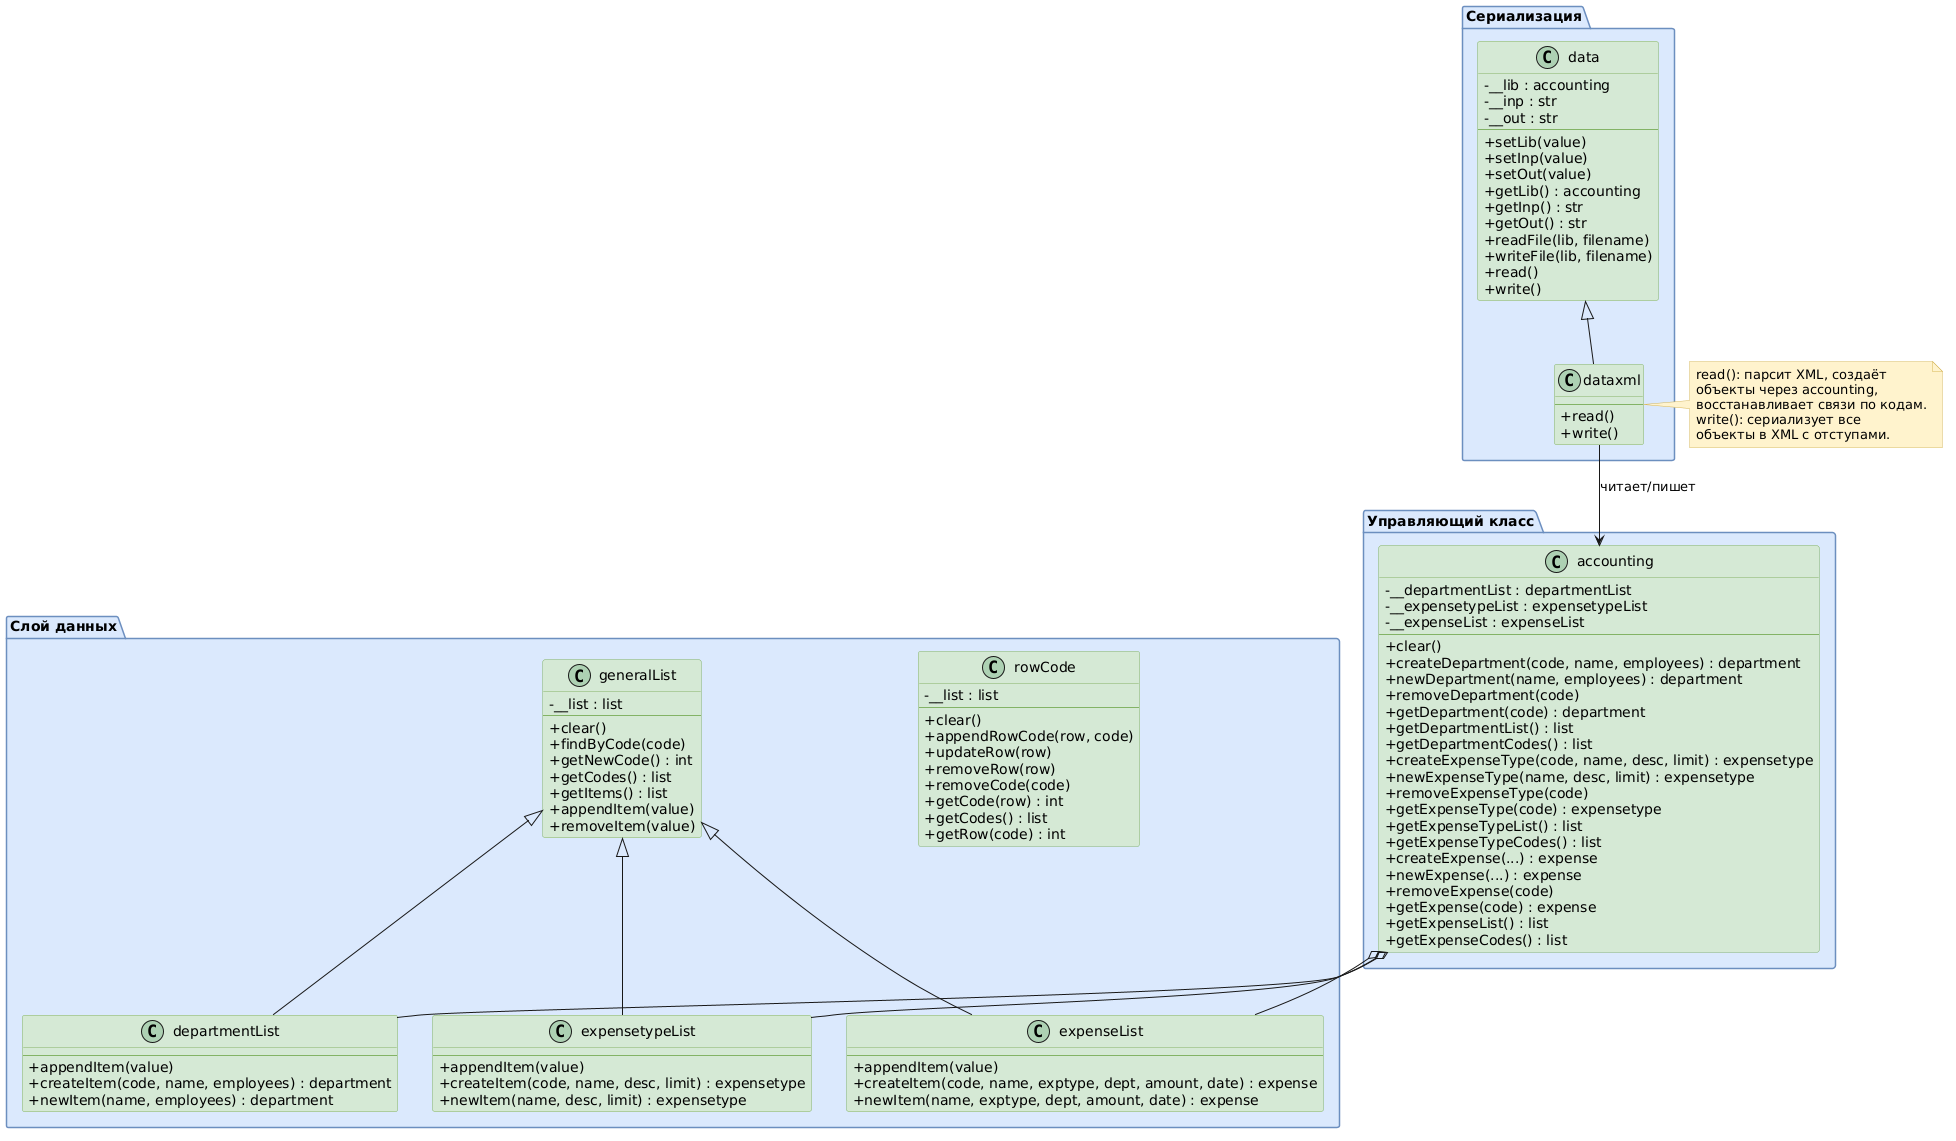
\includegraphics[width=0.9\textwidth]{screenshots/uml_data.png}
\caption{UML-диаграмма классов слоя данных}
\label{fig:uml2}
\end{figure}

\chapter{Задание 3: Реализация графического интерфейса PyQt5}

\section{Пояснение к выполнению Задания 3}

В соответствии с источниками, третий этап разработки заключается в создании полноценного графического интерфейса на базе библиотеки PyQt5. Архитектура GUI повторяет шаблон, продемонстрированный в учебных примерах \texttt{example4} и \texttt{example5}:

\begin{enumerate}
    \item \textbf{Базовые виджеты:} \texttt{libWidget} --- примесь для доступа к данным; \texttt{dbTableWidget} --- таблица с привязкой строк к кодам; \texttt{dbComboBox} --- выпадающий список с привязкой индексов к кодам.
    \item \textbf{Базовые формы:} \texttt{editForm} предоставляет сетку для размещения полей ввода и кнопок; \texttt{page} объединяет таблицу, форму редактирования и кнопки управления (добавить/изменить/удалить).
    \item \textbf{Специализированные виджеты:} Для каждой сущности создаются таблица, форма редактирования и страница. Для расхода дополнительно создаются комбо-боксы (\texttt{departmentCombo}, \texttt{expensetypeCombo}) для выбора связанных объектов.
    \item \textbf{Главное окно:} \texttt{tabWidget} объединяет страницы во вкладки; \texttt{mainWindow} добавляет меню (создать новый, открыть XML, сохранить XML).
\end{enumerate}

\subsection{Модуль \texttt{libwidget.py}}

Примесь (mixin), предоставляющая доступ к управляющему объекту данных \texttt{library}.

\lstinputlisting[label=lst:libwidget,caption=Модуль \texttt{libwidget.py} --- примесь для доступа к данным]{libwidget.py}

\subsection{Модуль \texttt{dbcombobox.py}}

Базовый выпадающий список, использующий \texttt{rowCode} для отображения индексов на коды объектов. Поддерживает методы \texttt{getCurrentCode()}, \texttt{setCurrentRec()} и динамическое обновление через \texttt{update()}.

\lstinputlisting[label=lst:dbcombobox,caption=Модуль \texttt{dbcombobox.py} --- выпадающий список с кодами]{dbcombobox.py}

\subsection{Модуль \texttt{dbtablewidget.py}}

Базовая таблица с автоматической привязкой строк к кодам объектов через \texttt{rowCode}. Метод \texttt{setData()} переопределяется в наследниках для заполнения таблицы конкретными данными.

\lstinputlisting[label=lst:dbtablewidget,caption=Модуль \texttt{dbtablewidget.py} --- таблица с кодами]{dbtablewidget.py}

\subsection{Модуль \texttt{editform.py}}

Базовая форма редактирования с сеточным размещением виджетов. Предоставляет методы \texttt{addLabel()}, \texttt{addNewWidget()}, \texttt{addLeftLayout()} для построения интерфейса, а также шаблонные методы \texttt{newClick()}, \texttt{editClick()}, \texttt{delClick()}, переопределяемые в наследниках.

\lstinputlisting[label=lst:editform,caption=Модуль \texttt{editform.py} --- базовая форма редактирования]{editform.py}

\subsection{Модуль \texttt{page.py}}

Базовая страница, объединяющая таблицу (\texttt{setTable}), форму редактирования (\texttt{setForm}) и кнопки управления (добавить, изменить, удалить). Метод \texttt{setConnect()} связывает сигналы кнопок с соответствующими обработчиками.

\lstinputlisting[label=lst:page,caption=Модуль \texttt{page.py} --- базовая страница с таблицей и формой]{page.py}

\subsection{Таблицы для сущностей}

Таблицы наследуются от \texttt{dbTableWidget} и переопределяют \texttt{setData()} для заполнения строк данными из соответствующих списков.

\subsubsection{Модуль \texttt{departmentstable.py}}

\lstinputlisting[label=lst:departmentstable,caption=Модуль \texttt{departmentstable.py} --- таблица отделов]{departmentstable.py}

\subsubsection{Модуль \texttt{expensetypestable.py}}

\lstinputlisting[label=lst:expensetypestable,caption=Модуль \texttt{expensetypestable.py} --- таблица видов расходов]{expensetypestable.py}

\subsubsection{Модуль \texttt{expensestable.py}}

\lstinputlisting[label=lst:expensestable,caption=Модуль \texttt{expensestable.py} --- таблица расходов]{expensestable.py}

\subsection{Комбо-боксы для выбора связанных объектов}

Для формы редактирования расхода созданы два специализированных выпадающих списка, которые заполняются данными из соответствующих списков и автоматически выбирают текущее значение при обновлении.

\subsubsection{Модуль \texttt{departmentcombo.py}}

\lstinputlisting[label=lst:departmentcombo,caption=Модуль \texttt{departmentcombo.py} --- комбо-бокс выбора отдела]{departmentcombo.py}

\subsubsection{Модуль \texttt{expensetypecombo.py}}

\lstinputlisting[label=lst:expensetypecombo,caption=Модуль \texttt{expensetypecombo.py} --- комбо-бокс выбора вида расхода]{expensetypecombo.py}

\subsection{Формы редактирования}

Формы наследуются от \texttt{editForm} и добавляют поля ввода, соответствующие атрибутам сущностей.

\subsubsection{Модуль \texttt{departmenteditform.py}}

\lstinputlisting[label=lst:departmenteditform,caption=Модуль \texttt{departmenteditform.py} --- форма редактирования отдела]{departmenteditform.py}

\subsubsection{Модуль \texttt{expensetypeeditform.py}}

\lstinputlisting[label=lst:expensetypeeditform,caption=Модуль \texttt{expensetypeeditform.py} --- форма редактирования вида расхода]{expensetypeeditform.py}

\subsubsection{Модуль \texttt{expenseeditform.py}}

Форма редактирования расхода содержит два комбо-бокса (\texttt{expensetypeCombo} и \texttt{departmentCombo}) для выбора вида расхода и отдела, поле для суммы (\texttt{QDoubleSpinBox}) и поле для даты (\texttt{QDateEdit} с календарём).

\lstinputlisting[label=lst:expenseeditform,caption=Модуль \texttt{expenseeditform.py} --- форма редактирования расхода]{expenseeditform.py}

\subsection{Страницы}

Каждая страница объединяет соответствующую таблицу и форму редактирования, а также устанавливает соединения между ними.

\subsubsection{Модуль \texttt{departmentpage.py}}

\lstinputlisting[label=lst:departmentpage,caption=Модуль \texttt{departmentpage.py} --- страница отделов]{departmentpage.py}

\subsubsection{Модуль \texttt{expensetypepage.py}}

\lstinputlisting[label=lst:expensetypepage,caption=Модуль \texttt{expensetypepage.py} --- страница видов расходов]{expensetypepage.py}

\subsubsection{Модуль \texttt{expensepage.py}}

\lstinputlisting[label=lst:expensepage,caption=Модуль \texttt{expensepage.py} --- страница расходов]{expensepage.py}

\subsection{Модуль \texttt{tabwidget.py}}

Виджет вкладок, объединяющий три страницы (отделы, виды расходов, расходы). При переключении вкладок обновляет все страницы.

\lstinputlisting[label=lst:tabwidget,caption=Модуль \texttt{tabwidget.py} --- виджет вкладок]{tabwidget.py}

\subsection{Модуль \texttt{mainwindow.py}}

Главное окно приложения. Содержит меню File с действиями: New (очистка данных), Open XML (загрузка из XML-файла), Save XML (сохранение в XML-файл). При открытии файла данные загружаются через \texttt{dataxml}, после чего все виджеты обновляются.

\lstinputlisting[label=lst:mainwindow,caption=Модуль \texttt{mainwindow.py} --- главное окно приложения]{mainwindow.py}

\subsection{Точка входа: \texttt{main.pyw}}

\lstinputlisting[label=lst:mainpyw,caption=Модуль \texttt{main.pyw} --- точка входа в приложение]{main.pyw}

\section{UML-диаграмма классов GUI}

На рисунке~\ref{fig:uml3} представлена диаграмма классов графического интерфейса, отражающая иерархию наследования виджетов и их отношения с классами данных.

\begin{figure}[H]
\centering
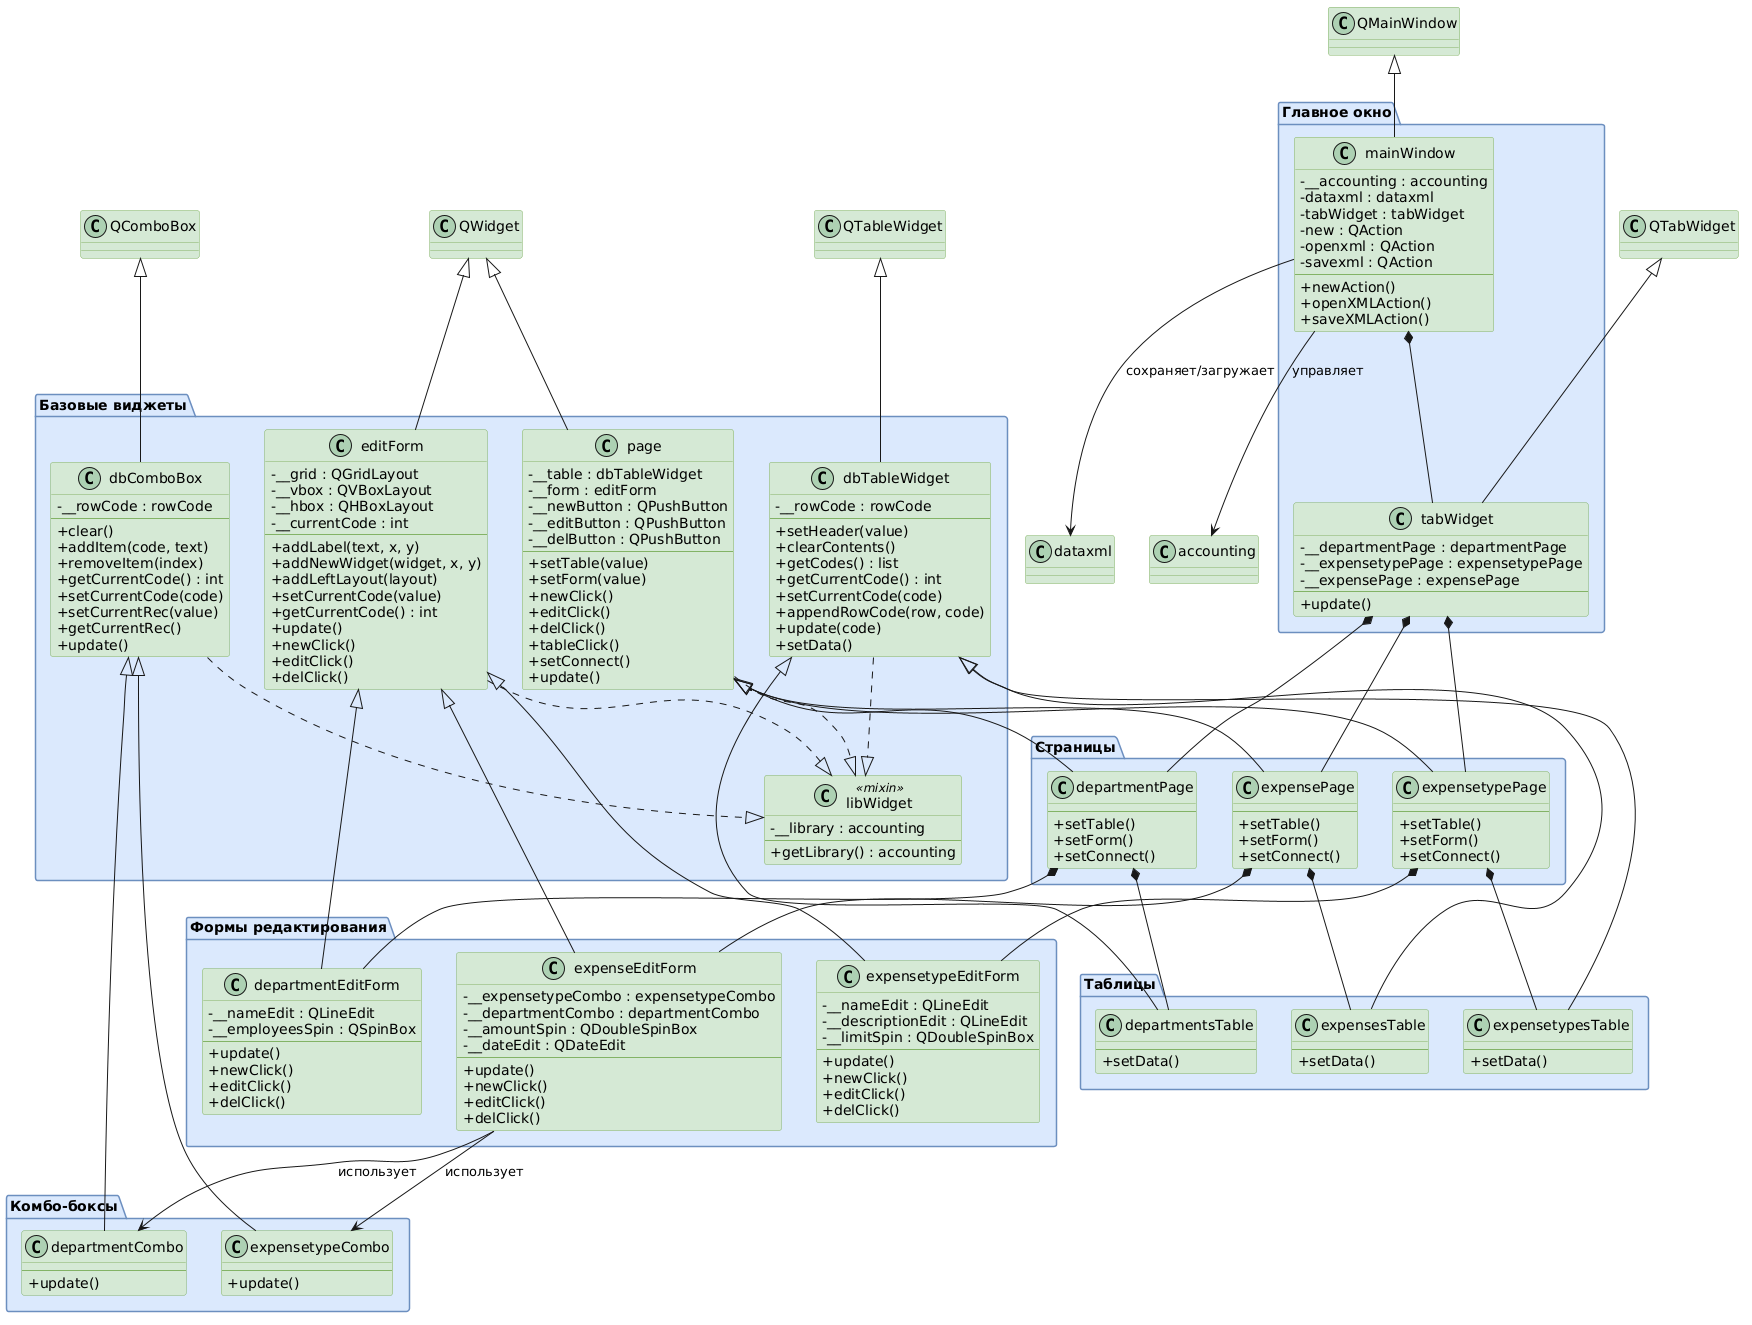
\includegraphics[width=\textwidth]{screenshots/uml_gui.png}
\caption{UML-диаграмма классов графического интерфейса}
\label{fig:uml3}
\end{figure}

\section{Результаты работы приложения}

При запуске приложения (\texttt{python main.pyw}) открывается главное окно с тремя вкладками. Пользователь может создать новую базу данных, загрузить данные из XML-файла или работать с существующими данными.

\subsection{Вкладка «Отделы»}

\begin{figure}[H]
\centering
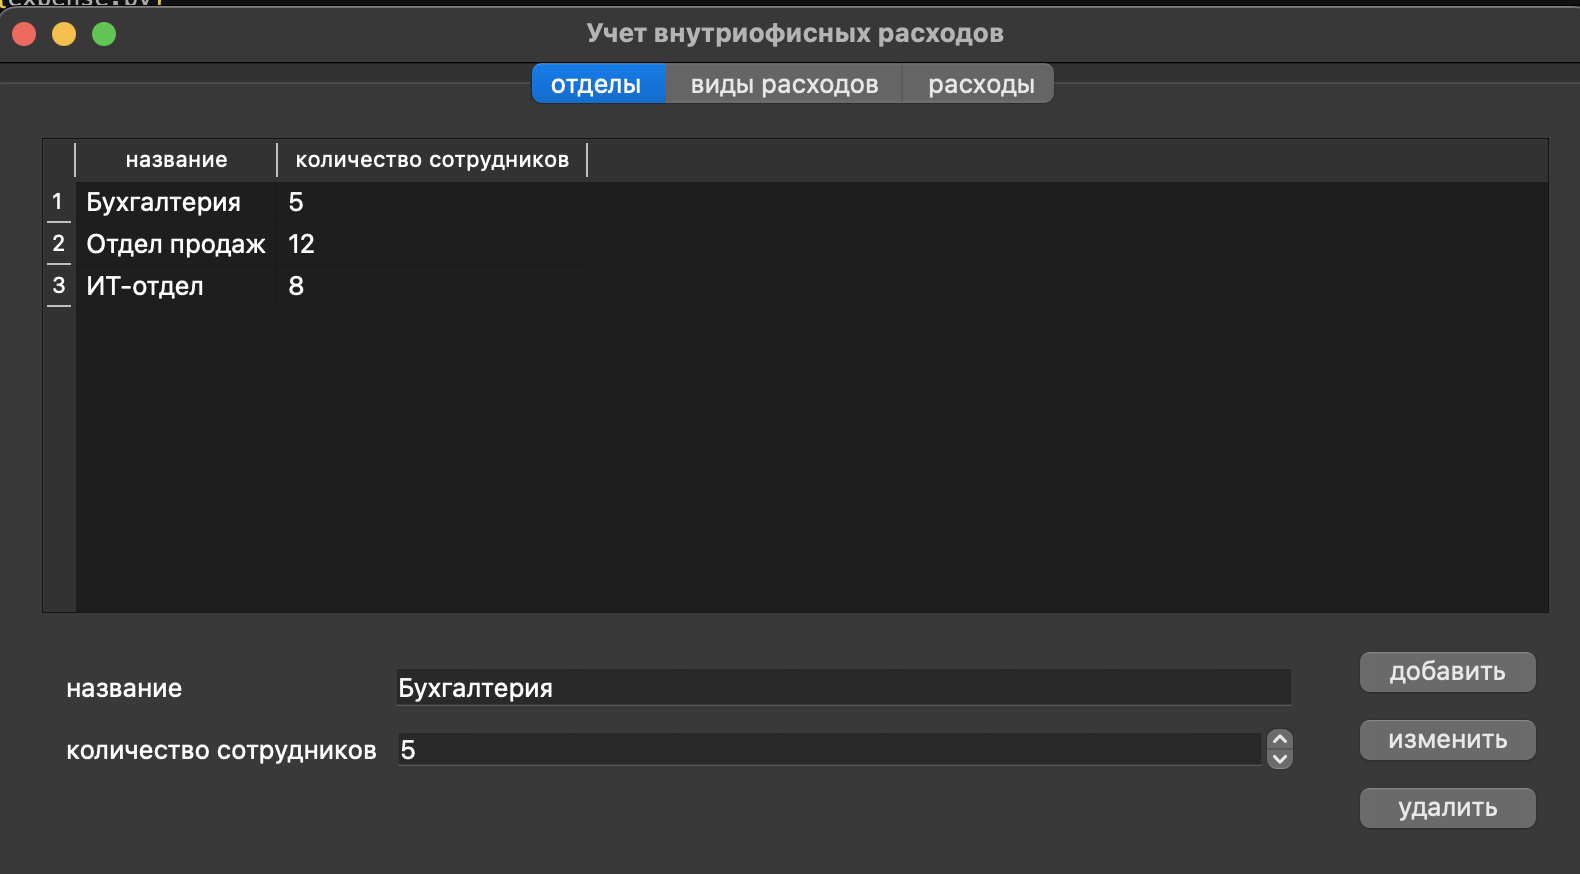
\includegraphics[width=\textwidth]{screenshots/screenshot_departments.png}
\caption{Вкладка «Отделы» с таблицей и формой редактирования}
\label{fig:scr_depts}
\end{figure}

На рисунке~\ref{fig:scr_depts} показана вкладка «Отделы». В верхней части расположена таблица со списком отделов (название, количество сотрудников). В нижней части --- форма редактирования, позволяющая добавлять новые отделы, изменять существующие и удалять их.

\subsection{Вкладка «Виды расходов»}

\begin{figure}[H]
\centering
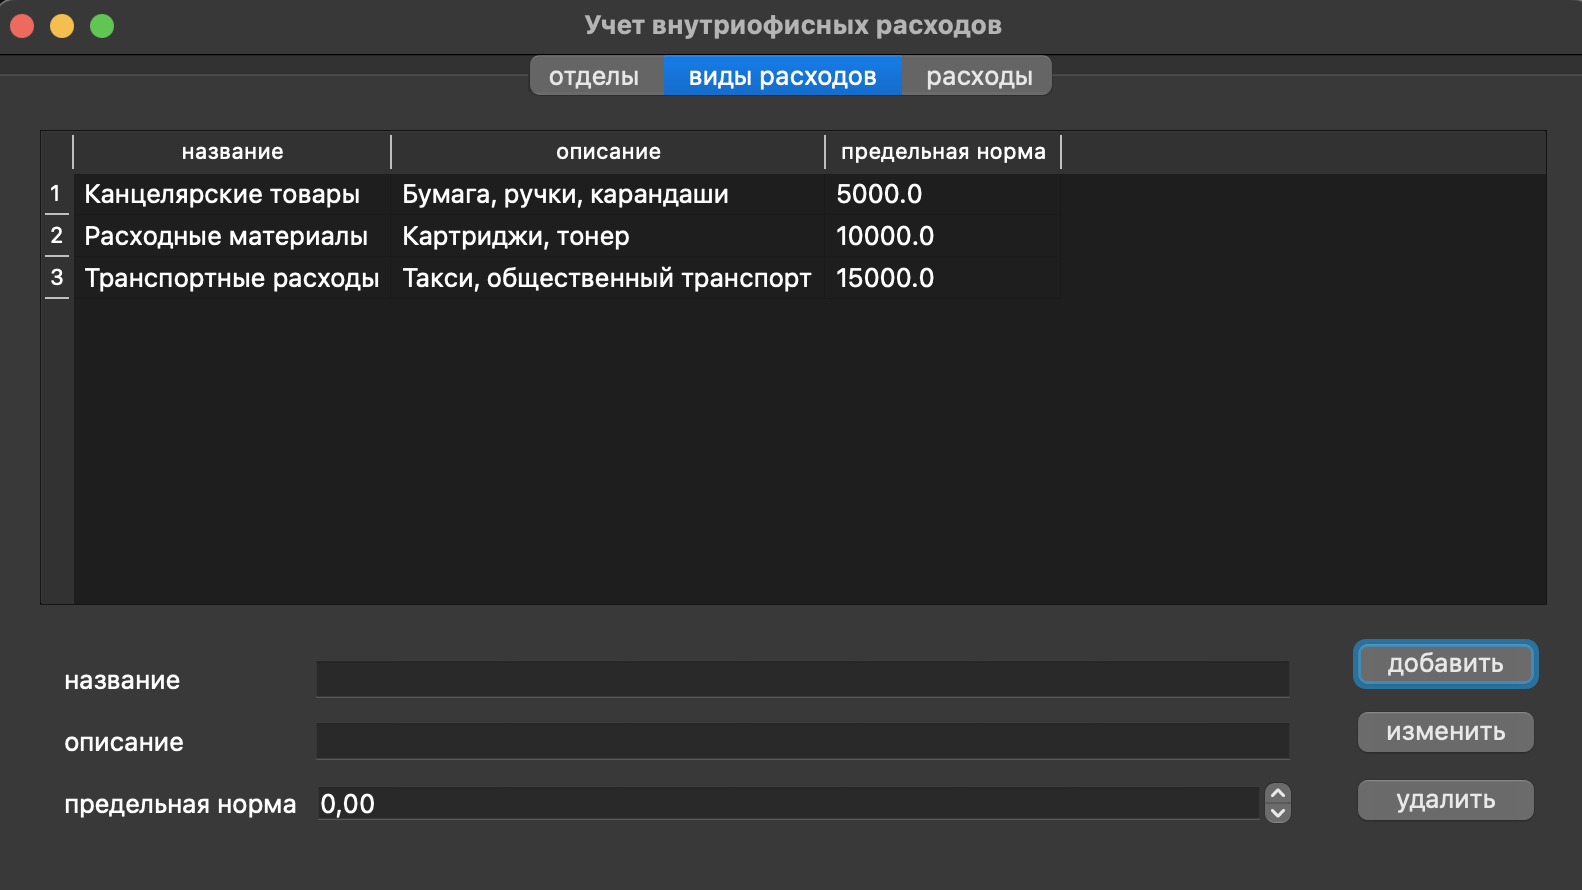
\includegraphics[width=\textwidth]{screenshots/screenshot_expensetypes.png}
\caption{Вкладка «Виды расходов» с таблицей и формой редактирования}
\label{fig:scr_types}
\end{figure}

На рисунке~\ref{fig:scr_types} показана вкладка «Виды расходов». Форма редактирования содержит поля: название, описание и предельная норма (с использованием \texttt{QDoubleSpinBox}).

\subsection{Вкладка «Расходы»}

\begin{figure}[H]
\centering
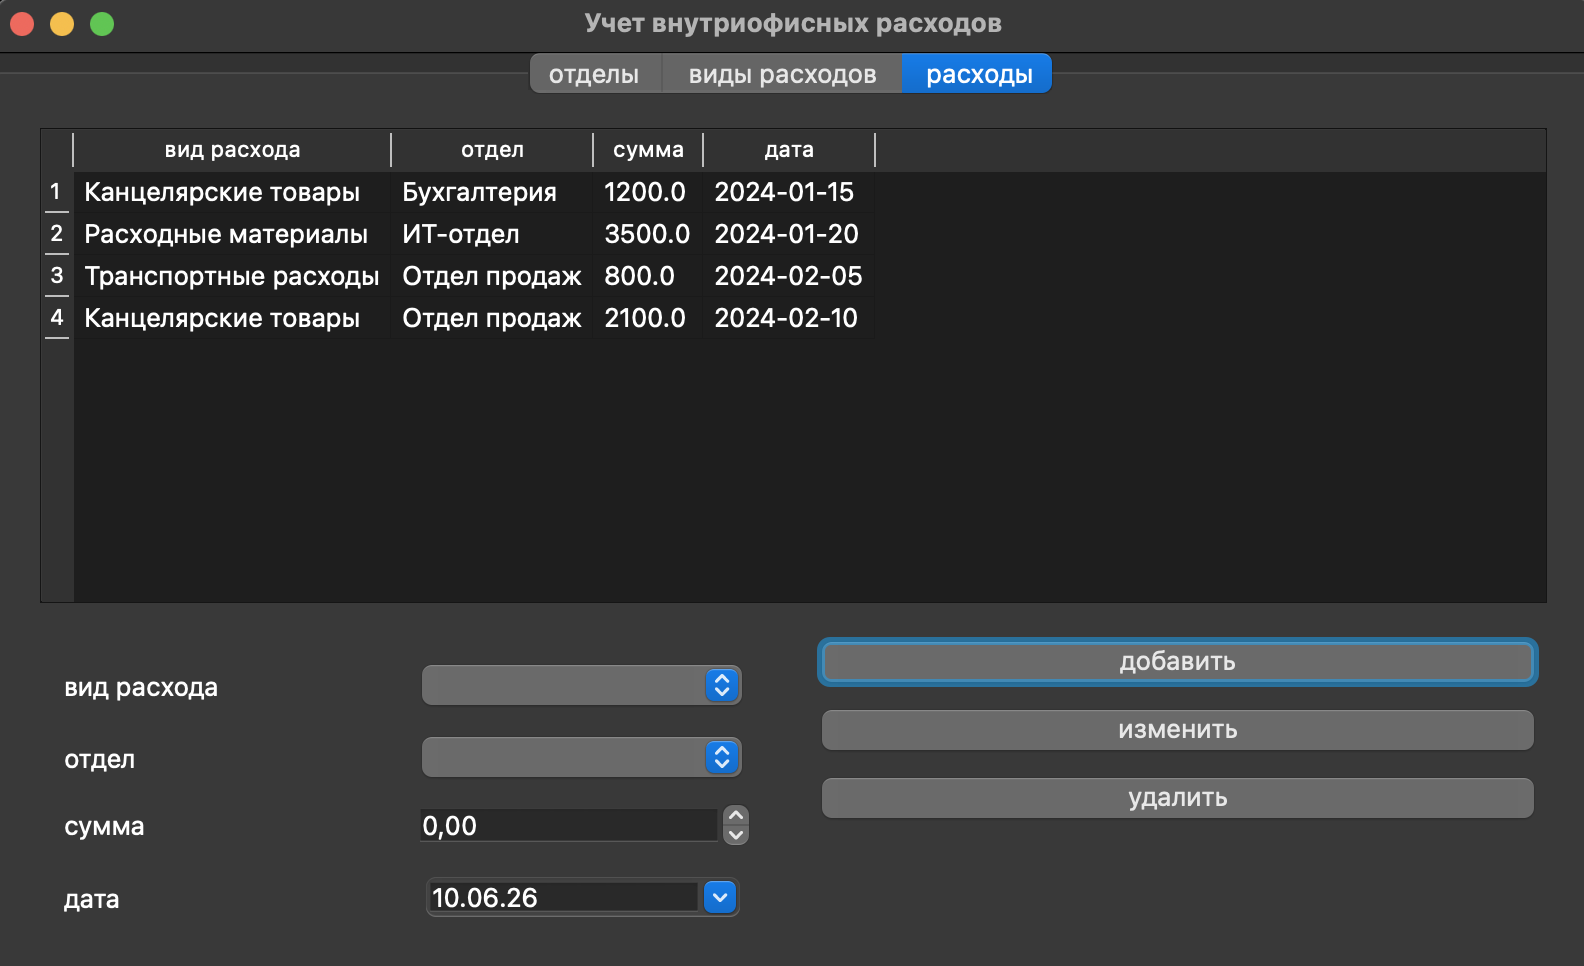
\includegraphics[width=\textwidth]{screenshots/screenshot_expenses.png}
\caption{Вкладка «Расходы» с таблицей и формой редактирования}
\label{fig:scr_expenses}
\end{figure}

На рисунке~\ref{fig:scr_expenses} показана вкладка «Расходы». Форма редактирования содержит выпадающие списки для выбора вида расхода и отдела, поле ввода суммы и календарь для выбора даты.

\subsection{Загрузка данных из XML}

\begin{figure}[H]
\centering
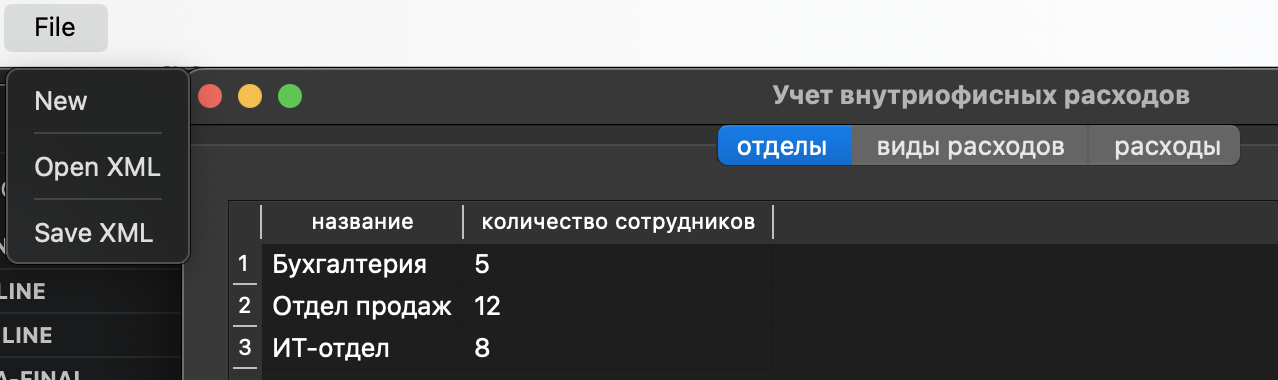
\includegraphics[width=\textwidth]{screenshots/screenshot_open_xml.png}
\caption{Загрузка данных из XML-файла}
\label{fig:scr_open}
\end{figure}

На рисунке~\ref{fig:scr_open} показан результат загрузки данных из файла \texttt{data.xml} через меню File → Open XML. После загрузки все три вкладки заполняются данными, и связи между расходами, отделами и видами расходов восстанавливаются корректно.

\subsection{Сохранение данных в XML}

\begin{figure}[H]
\centering
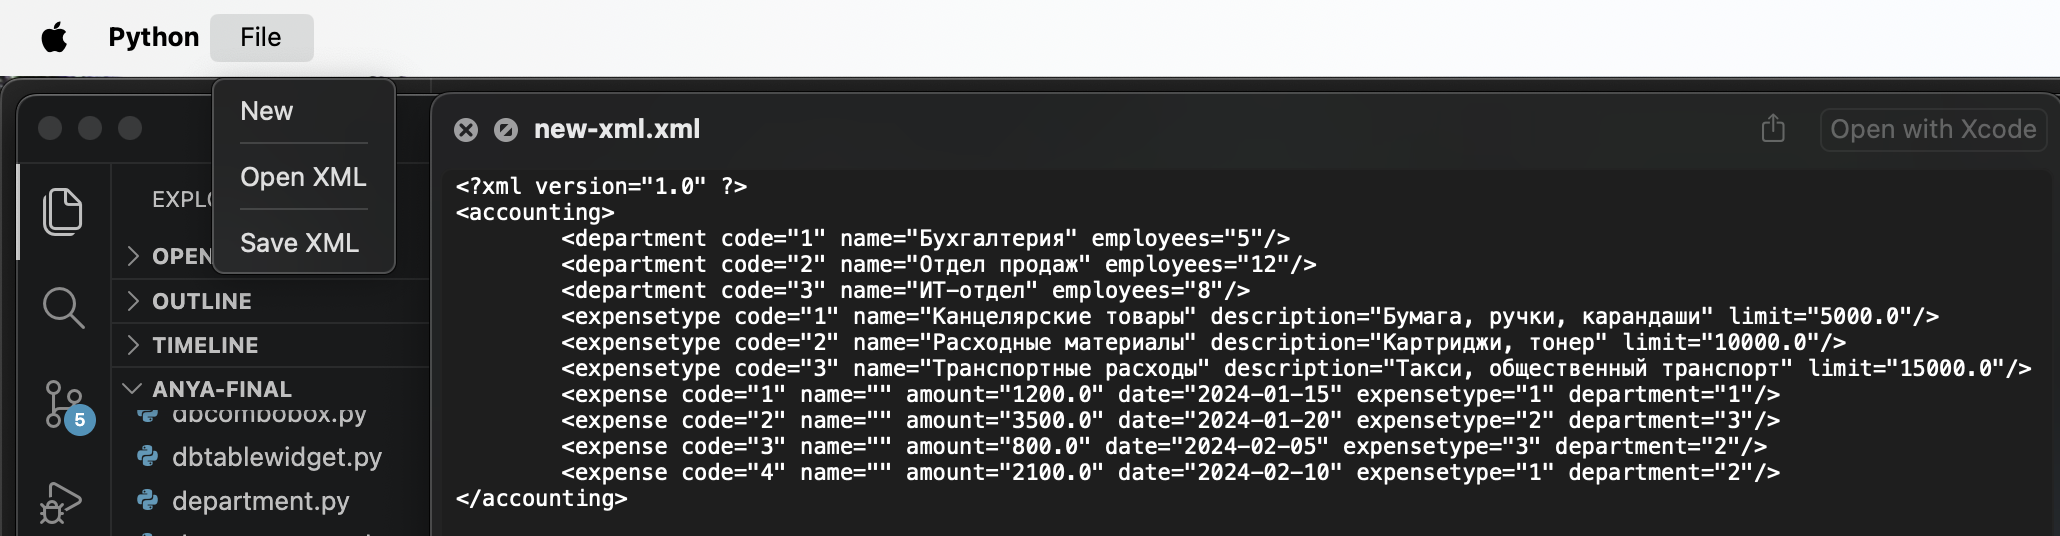
\includegraphics[width=\textwidth]{screenshots/screenshot_save_xml.png}
\caption{Сохранение данных в XML-файл}
\label{fig:scr_save}
\end{figure}

На рисунке~\ref{fig:scr_save} показан процесс сохранения данных. При выборе File → Save XML открывается диалог сохранения файла, после чего данные записываются в формат XML с правильным форматированием и кодировкой UTF-8.

\chapter{Заключение}

В результате выполнения курсовой работы разработано приложение на языке Python с графическим интерфейсом PyQt5 для учёта внутриофисных расходов. Приложение реализует:

\begin{itemize}
    \item Объектно-ориентированную модель предметной области с тремя сущностями (Отдел, Вид расхода, Расход), построенную на принципах наследования и агрегации.
    \item Систему хранения данных на основе специализированных списков с централизованным управлением через класс \texttt{accounting}.
    \item Полноценный графический интерфейс с таблицами, формами редактирования, выпадающими списками для выбора связанных объектов и календарём для выбора даты.
    \item Поддержку сохранения и загрузки данных в формате XML с использованием библиотеки \texttt{xml.dom.minidom}.
    \item Архитектуру, полностью соответствующую шаблонам, представленным в учебных примерах \texttt{example4} и \texttt{example5}.
\end{itemize}

Приложение готово к использованию в бухгалтерии частной фирмы для отслеживания внутриофисных расходов сотрудников.

\vspace{10pt}
Общий объём исходного кода составляет 31 файл (около 800 строк), что демонстрирует масштабируемость выбранной архитектуры и её пригодность для дальнейшего расширения (добавление поддержки JSON, SQLite и других форматов хранения).

\end{document}
